\chapter[Theory]{Theory of Optical Trapping}\label{ch:theory}

\lipsum[1-5]

\begin{figure}[htp]
  \centering
  \includegraphics[width=0.8\linewidth]{T_quadrant_Intensity.pdf}
  \caption{Caption}
  \label{fig:T_quadrant_Intensity}
\end{figure}

\lipsum[1-5]
\begin{figure}
  \centering
  \begin{subfigure}[b]{0.3\textwidth}
    \centering
    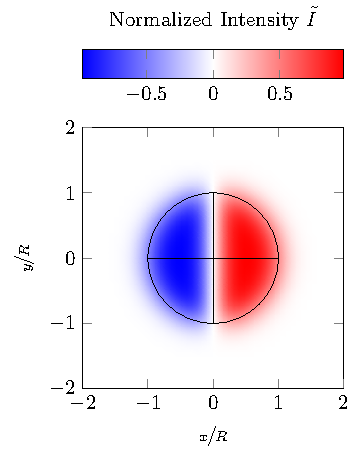
\includegraphics[width=\textwidth]{T_xQPD.pdf}
    \caption{Caption}
    \label{fig:T_xQPD}
  \end{subfigure}
  \hfill
  \begin{subfigure}[b]{0.3\textwidth}
    \centering
    \includegraphics[width=\textwidth]{T_yQPD.pdf}
    \caption{Caption}
    \label{fig:T_yQPD}
  \end{subfigure}
  \hfill
  \begin{subfigure}[b]{0.3\textwidth}
    \centering
    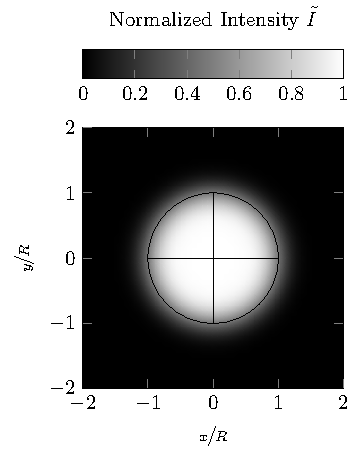
\includegraphics[width=\textwidth]{T_totalQPD.pdf}
    \caption{Caption}
    \label{fig:T_totalQPD}
  \end{subfigure}
  \caption{QPDs}
  \label{fig:QPDs}
\end{figure}

\lipsum[1-5]

\begin{figure}[htp]
  \centering
  \includegraphics[]{T_Snells_Law.pdf}
  \caption{Caption}
  \label{fig:T_snell}
\end{figure}

\lipsum[1-5]

\begin{figure}
  \centering
  \begin{subfigure}[b]{0.45\textwidth}
    \centering
    \includegraphics[]{T_gamma.pdf}
    \caption{Caption}
    \label{fig:T_gamma}
  \end{subfigure}
  \hfill
  \begin{subfigure}[b]{0.45\textwidth}
    \centering
    \includegraphics[]{T_theta_i.pdf}
    \caption{Caption}
    \label{fig:T_theta_i}
  \end{subfigure}
  \caption{angles}
  \label{fig:T_gamma_theta}
\end{figure}

\lipsum[1-5]

\begin{figure}[htp]
  \centering
  \includegraphics[]{T_voltages_over_x.pdf}
  \caption{Fresnel}
  \label{fig:T_voltages_over_x}
\end{figure}

\lipsum[1-5]

\begin{figure}[htp]
  \centering
  \includegraphics[]{T_fresnel.pdf}
  \caption{Fresnel}
  \label{fig:T_fresnel}
\end{figure}

\lipsum[1-5]

\begin{figure}[htp]
  \centering
  \includegraphics[]{T_Angles.pdf}
  \caption{Caption}
  \label{fig:T_angles}
\end{figure}

\lipsum[1-5]

\begin{figure}[htp]
  \centering
  \includegraphics[]{T_Ray_Particle.pdf}
  \caption{Caption}
  \label{fig:T_ray_particle}
\end{figure}
